\documentclass[aip, jcp, reprint, onecolumn, nofootinbib]{revtex4-2}

\bibliographystyle{apsrev4-2}

\usepackage{physics}
\usepackage{amsmath}
\usepackage{amssymb}
\usepackage{mathtools}
\usepackage{graphicx}
\usepackage{dcolumn}
\usepackage[colorlinks=true, linkcolor=black, urlcolor=blue, citecolor=black, anchorcolor=black]{hyperref}

%supplementary figs
\renewcommand{\thefigure}{S\arabic{figure}}
\renewcommand{\thetable}{S\arabic{table}}
\renewcommand\theequation{S\arabic{equation}}
\renewcommand*{\thepage}{S\arabic{page}}

\graphicspath{{"figures/"}}
\begin{document}
%Title of paper
\title{Supporting Information for Coherent IR-Hyper-Raman Four Wave Mixing Spectroscopy}


\author{Ryan P. McDonnell} 
\author{Daniel D. Kohler}
\author{John C. Wright} \email{wright@chem.wisc.edu}

\affiliation{Department of Chemistry, 
        University of Wisconsin - Madison, 
        Madison, Wisconsin 53706, 
        United States of America}

\date{\today}

\maketitle
\tableofcontents
\clearpage


\section{Evaluating Herzberg-Teller Integrals for Harmonic Wells of Identical Curvature}
In this section, we discuss the evaluation of Herzberg-Teller integrals, in the limit of no Duschinsky coupling, when the ground and first excited state are harmonic wells of identical curvature.\cite{HerzbergTeller1933, Duschinsky1937}
We investigate the one dimensional case using the Hamiltonian described in the main text, $H = H_g |g) \left(g| + H_e |e\right) (e|$, where
\begin{subequations}\label{Hamiltonian}
	\begin{equation}
		H_g = \frac{\hbar \omega }{2} \left(p^2 + q^2 \right)
	\end{equation}
	and
	\begin{equation}
		H_e = \frac{\hbar \omega }{2} \left(p^2 +  (q-\Delta)^2 \right) + \hbar \omega_{eg}.
	\end{equation} 
\end{subequations}
Here, $p,q$ are the dimensionless conjugate normal mode coordinates, $\hbar\omega_{eg}$ is the energy difference between $H_e$ and $H_g$, and $\Delta$ is the dimensionless offset of the excited state surface relative to the ground state.
Franck-Condon factors and Herzberg-Teller integrals are often evaluated in position space using known solutions to the Harmonic Oscillator Hamiltonian, 
\begin{equation}
	\psi_m(q) = \langle q | m \rangle = N(m) H_m(q) \exp(-q^2/2),
\end{equation}
where $N(m) = (m! \ 2^m \pi^{\frac{1}{2}})^{-\frac{1}{2}}$ is the normalization factor and $H_m$ is the m$^{th}$ Hermite Polynomial.\cite{RN230}
We begin by generating an expression for $\mel{\tilde{n}}{q^k}{m}$, as this will resolve into Franck-Condon factors for $k = 0$ and Herzberg-Teller integrals for $k=1$.
As in the main text, $\{\ket{\tilde{a}}\}$ are vibrational states on the first excited state $|e)$ and $\{\ket{b}\}$ are vibrational states on the ground state $|g)$.

By letting $\ket{m}$ belong to the ground state surface $|g)$ and $\ket{\tilde{n}}$ belong to the first excited surface $|e)$, we write
\begin{equation}
\begin{split}
		\mel{\tilde{n}}{q^k}{m} &= \int_{-\infty}^\infty \mathrm{d}q \psi^*_n(q-\Delta) q^k \psi_m(q)\\
		&= \int_{-\infty}^\infty \mathrm{d}q N(n) N(m) H_n(q-\Delta) \exp(-\frac{(q - \Delta)^2}{2}) q^k H_m(q) \exp(-\frac{q^2}{2}),
\end{split}
\end{equation}
where $k=0$ corresponds to a Franck-Condon factor and $k=1$ refers to a Herzberg-Teller integral.
Introducing $\tilde{N} \equiv N(n)N(m)$ and slightly rearranging, we see
\begin{equation}\label{key}
	\mel{\tilde{n}}{q^k}{m} = \tilde{N} \exp(-\frac{\Delta^2}{2}) \int_{-\infty}^\infty \mathrm{d}q H_n(q-\Delta) q^k H_m(q) \exp(-q^2 + q\Delta)
\end{equation}
This is the key result.
While integrals of form \autoref{key} can be computed straightforwardly using mathematical packages such as \texttt{Mathematica} or \texttt{SymPy}, \cite{Mathematica, sympy} it is a useful exercise in Gaussian integral manipulation to evaluate Herzberg-Teller or Franck-Condon integrals.
As a side note, \autoref{key} explicitly shows
\begin{subequations}
	\begin{equation}
		\lim_{\Delta \rightarrow 0} \langle \tilde{n} | m \rangle = \langle n | m \rangle = \delta_{n,m}
	\end{equation}
and
	\begin{equation}
	\lim_{\Delta \rightarrow 0} \mel{\tilde{n}}{q}{m} = \mel{{n}}{q}{m} = \sqrt{\frac{1}{2}} \left(\sqrt{m}\delta_{n,m-1} + \sqrt{m+1} \delta_{n,m+1}\right)
	\end{equation}
\end{subequations}
i.e., as the offset vanishes, the normal harmonic oscillator selection rules are obtained, the expected result, where $\delta$ is the Kronecher delta.

It is well known that the Hermite polynomials $H_v(q)$ are linear combinations of $q^w$, $w \in \mathbf{N}$. 
Thus, evaluating \autoref{key} for arbitrary $m,n,k$ values resolves into evaluating sums of integrals of the form
\begin{equation}\label{integral}
	\int_{-\infty}^\infty \mathrm{d}q \ q^w \exp(-q^2 + q\Delta)
\end{equation}
When $w=0$, the result follows by completing the square:\footnote{$\int_{-\infty}^{\infty} \mathrm{d}x \exp(-(x-a)^2) = \sqrt{\pi}$}
\begin{equation}
	\begin{split}
		\int_{-\infty}^\infty \mathrm{d}q \exp(-q^2 + q\Delta) &= \int_{-\infty}^\infty \mathrm{d}q \exp(-(q^2 - q\Delta +\frac{\Delta^2}{4} - \frac{\Delta^2}{4}))\\
		&= \exp(\frac{\Delta^2}{4}) \int_{-\infty}^\infty \mathrm{d}q \exp(-(q - \frac{\Delta}{2})^2) \\
		&= \sqrt{\pi} \exp(\frac{\Delta^2}{4})
	\end{split}
\end{equation}
 For $w \neq 0$, \autoref{integral} is evaluated through repeated use of a well-known Gaussian identity
\begin{equation}\label{identity}
	\int_{-\infty}^\infty \mathrm{d}q \ q^w \exp(-q^2 + q\Delta) = \partial_{\Delta} \int_{-\infty}^\infty \mathrm{d}q \ q^{w-1} \exp(-q^2 + q\Delta)
\end{equation}

We now have the background needed to calculate $\mel{\tilde{1}}{q}{0}$ for an arbitrary offset $\Delta$.
We note that Myers et al. have developed a general expression to evaluate Franck-Condon factors for two displaced harmonic wells of arbitrary curvature,\cite{Myers1982} so we focus our attention onto Herzberg-Teller integrals, which are not commonly tabulated.
Starting with \autoref{key},
\begin{equation}
\begin{split}
	\mel{\tilde{1}}{q}{0} = \tilde{N} \exp(-\frac{\Delta^2}{2}) \int_{-\infty}^\infty \mathrm{d}q H_1(q-\Delta) q H_0(q) \exp(-q^2 + q\Delta)
\end{split}
\end{equation}
Using $H_0(q) = 1$ and $H_1(q) = 2q$,
\begin{equation}\label{HT10}
	\begin{split}
		\mel{\tilde{1}}{q}{0} &= \tilde{N} \exp(-\frac{\Delta^2}{2}) \int_{-\infty}^\infty \mathrm{d}q \ 2(q - \Delta) q \exp(-q^2 + q\Delta)\\
		&= 2\tilde{N} \exp(-\frac{\Delta^2}{2}) \int_{-\infty}^\infty \mathrm{d}q \ (q^2 - q \Delta) \exp(-q^2 + q\Delta)\\
		&=  2\tilde{N} \exp(-\frac{\Delta^2}{2}) \left(\int_{-\infty}^\infty \mathrm{d}q \ q^2 \exp(-q^2 + q\Delta) - \Delta \int_{-\infty}^\infty \mathrm{d}q \ q \exp(-q^2 + q\Delta) \right)
	\end{split}
\end{equation}
These integrals are now easily evaluated using \autoref{identity}:
\begin{subequations}\label{evalGaussians}
	\begin{equation}
		\begin{split}
					\int_{-\infty}^\infty \mathrm{d}q \ q \exp(-q^2 + q\Delta) &= \partial_{\Delta} \left(\sqrt{\pi} \exp(\frac{\Delta^2}{4})\right)\\
					& = \sqrt{\pi} \frac{\Delta}{2} \exp(\frac{\Delta^2}{4})
		\end{split}
	\end{equation}
giving
\begin{equation}
	\begin{split}
		\int_{-\infty}^\infty \mathrm{d}q \ q^2 \exp(-q^2 + q\Delta) &= \partial_{\Delta} \left(\sqrt{\pi} \left(\frac{\Delta}{2} \exp(\frac{\Delta^2}{4})\right)\right)\\
		& =\sqrt{\pi} \left(\frac{1}{2}\exp(\frac{\Delta^2}{4}) + \frac{\Delta^2}{4} \exp(\frac{\Delta^2}{4})\right)
	\end{split}
\end{equation}
\end{subequations}
With $\tilde{N} = N(1)*N(0) = (1! \ 2^1 \pi^{\frac{1}{2}})^{-\frac{1}{2}} * (0! \ 2^0 \pi^{\frac{1}{2}})^{-\frac{1}{2}} = \sqrt{1/2\pi}$ and substituting the results of \autoref{evalGaussians} into \autoref{HT10}, 
\begin{equation}
	\mel{\tilde{1}}{q}{0} = \sqrt{\frac{1}{2}} (1 - \frac{\Delta^2}{2}) \exp(\frac{-\Delta^2}{4})
\end{equation}
The evaluation of other Herzberg-Teller integrals follows a similar process. 


\section{Impact of $\Delta$ on $A,B$ Terms in HDFG Spectra}
In the main text, the potential well offset ($\Delta$) was taken as $\Delta = 0.5$.
Here, we vary $\Delta$ to investigate its impact on the structure of the $\abs{A+B}$ spectrum.
The relevant Franck-Condon factors and Herzberg-Teller integrals, assuming identical curvature and no Duschinsky coupling, are plotted in \autoref{fig:fcht} as a function of offset, $\Delta$.

\begin{figure}[!htbp]
	\centering
	\includegraphics[width=6.675in]{figures/fcht.png}
	\caption{Plots of select (a) Franck-Condon factors and (b) Herzberg-Teller integrals relevant to this manuscript as a function of offset, $\Delta$.} 
	\label{fig:fcht}
\end{figure}

It is clear from \autoref{fig:fcht} that the HDFG spectrum will have a significant dependence upon $\Delta$, even for small deviations from complete overlap. 
To this end, we first investigate the impact of $\Delta$ on a vibrational mode with a fundamental frequency 1600 cm$^{-1}$ and linewidth of 400 cm$^{-1}$ (\autoref{fig:chgdelta}). 

\begin{figure}[!htbp]
	\centering
	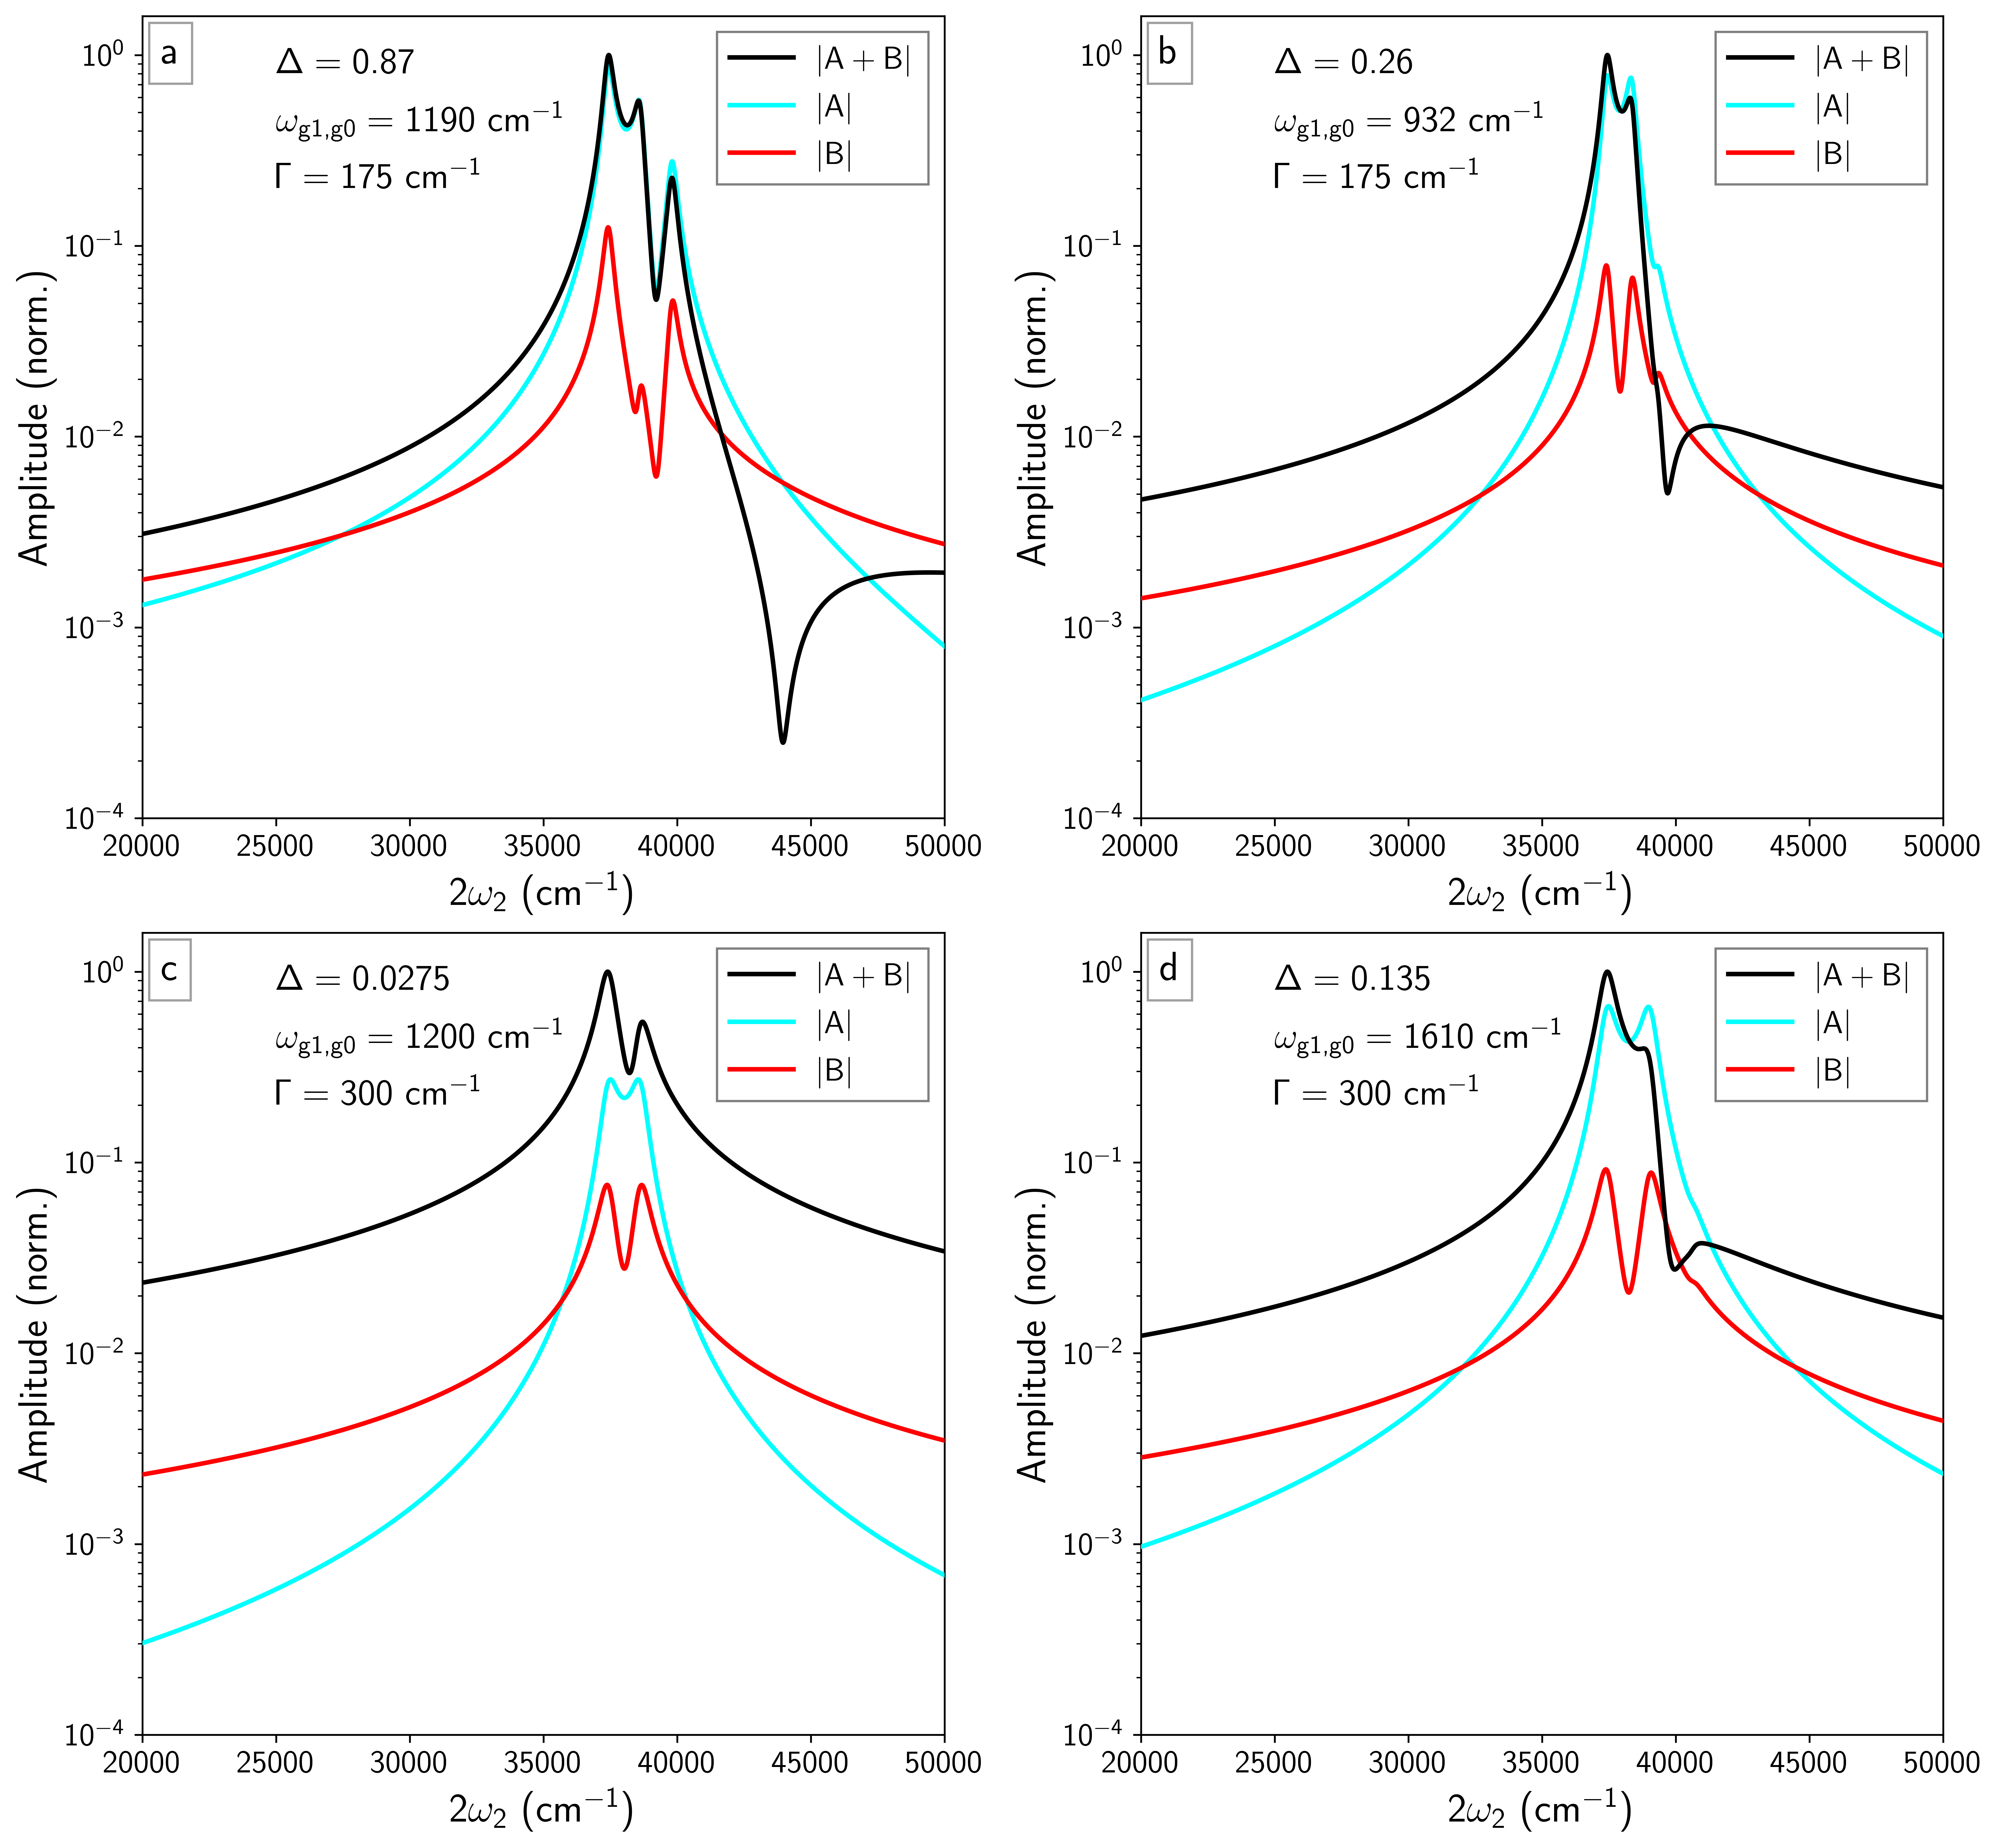
\includegraphics[width=6.675in]{figures/changedelta.png}
	\caption{Plots of select (a) Franck-Condon factors and (b) Herzberg-Teller integrals relevant to this manuscript as a function of offset, $\Delta$.} 
	\label{fig:chgdelta}
\end{figure}
\section{Evaluation of Equation 14}
In this section, the integral
\begin{equation}
	\begin{split}
		\gamma_{ijkl} &= \int_{-\infty}^\infty \mathrm{d}\xi P(\xi) \gamma_{ijkl}(\xi)\\
		&=\frac{\sigma}{\pi}\int_{-\infty}^\infty \mathrm{d}\xi \frac{1}{\sigma^2 + \xi^2} \frac{\gamma_0}{\Delta_{ga}(\xi)\Delta_{ba}(\xi)} \\
		&= \frac{\gamma_0 \sigma}{\pi} \int_{-\infty}^\infty \mathrm{d}\xi\frac{1}{(\xi + i\sigma)(\xi - i\sigma)} \frac{1}{\Delta_{ga}(0) - \xi} \frac{1}{\Delta_{ba}(0) + c\xi}\\
	\end{split}
\end{equation}
is evaluated using Contour integration.
\begin{figure}[!htbp]
	\centering
	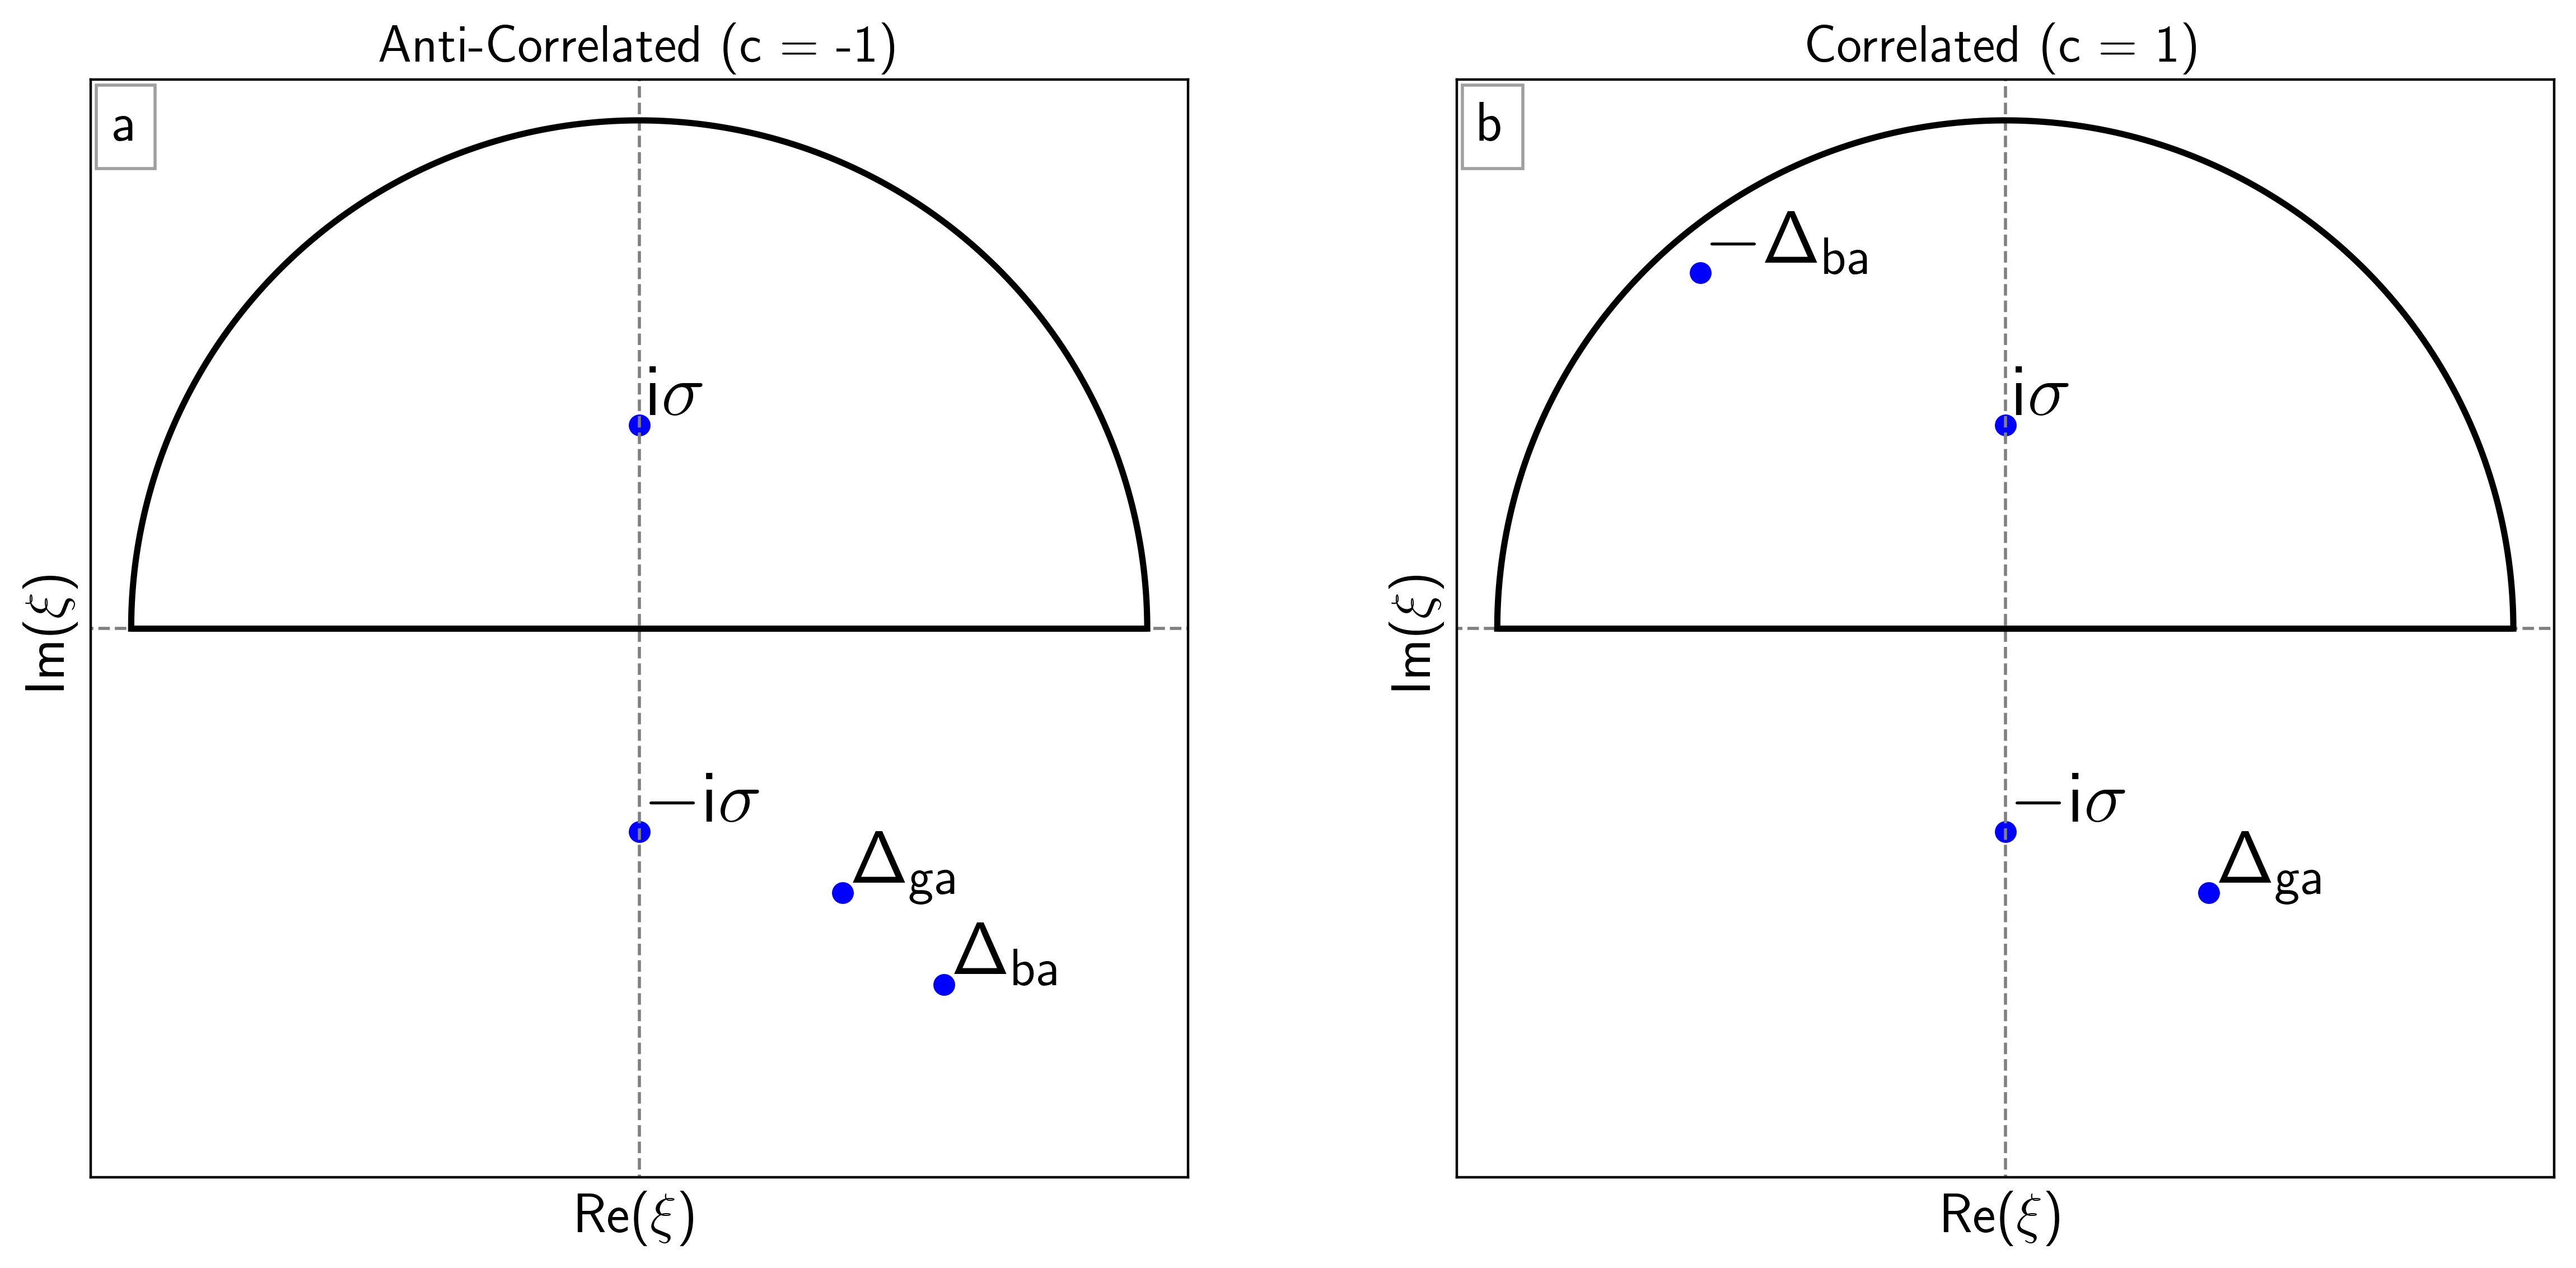
\includegraphics[width=3.375in]{figures/corr_contour.png}
	\caption{Poles (black dots) and contour (blue line) used to evaluate \autoref{integraly} for (a) anti-correlated and (b) correlated modes.} 
	\label{fig:contours}
\end{figure}
\subsection{Anti-correlated Modes}
For anti-correlated modes, the poles are situated in the complex plane as shown in \autoref{fig:contours}a.
Since \autoref{integraly} is evaluated along the real axis, one can choose to evaluate the contour in the upper or lower half of the complex plane.
Since evaluating the residues in the upper or lower half of the complex plane yields the same result for \autoref{integraly}, we choose the contour which wraps around the least number of poles.
It is clear for c = -1 that there are four poles: $\pm i \sigma, \Delta_{ga}(0), \Delta_{ba}(0)$. 
Following \autoref{fig:contours}, the contour that wraps the upper half of the complex plane has only one pole, $i \sigma$; as such, we choose to evaluate \autoref{integraly} in the upper half of the complex plane for the case of anti-correlated modes through the residue theorem as
\begin{widetext}
	\begin{equation}
		\begin{split}
			\int_{-\infty}^\infty \mathrm{d}\xi P(\xi) \gamma_{ijkl}(\xi) &= 2\pi i \sum_k \lim_{\xi \rightarrow \xi_k} P(\xi) \gamma_{ijkl}(\xi) (\xi - \xi_k)\\
			&= 2\pi i \frac{\gamma_0 \sigma}{\pi} \lim_{\xi \rightarrow i\sigma} \frac{1}{(\xi + i\sigma)(\xi - i\sigma)} \frac{1}{\Delta_{ga}(0) - \xi} \frac{1}{\Delta_{ba}(0) - \xi} (\xi - i \sigma)\\
			&= 2 \gamma_0 \sigma i \lim_{\xi \rightarrow i\sigma} \frac{1}{\xi + i\sigma} \frac{1}{\Delta_{ga}(0) - \xi} \frac{1}{\Delta_{ba}(0) - \xi}\\
			&= 2\gamma_0 \sigma i \frac{1}{2i\sigma} \frac{1}{\Delta_{ga}(0) - i\sigma} \frac{1}{\Delta_{ba}(0) - i\sigma}\\
			&= \frac{\gamma_0}{\Delta_{ga}(i\sigma)\Delta_{ba}(i \sigma)}\\
		\end{split}
	\end{equation}
\end{widetext}

\subsection{Correlated Modes}
For correlated modes, the poles are situated in the complex plane as shown in \autoref{fig:contours}.
It is clear that no matter which contour is chosen, there is a contribution to the final integral from either $\Delta_{ba}(0)$ or $\Delta_{ga}(0)$. 
For the below calculation, we choose to evaluate along the contour in the bottom half of the complex plane, i.e., the poles ($\xi_k$) are $-i\sigma, \Delta_{ga}$.
We stress that since the integral is evaluated over $\mathbb{R}$ and there are no degenerate poles, the results below can be obtained by evaluating the contour which wraps around the poles $i\sigma, \Delta_{ba}$. 
Since the $\xi_k$ are nondegenerate,
\begin{widetext}
	\begin{equation}
		\begin{split}
			\int_{-\infty}^\infty \mathrm{d}\xi P(\xi) \gamma_{ijkl}(\xi) &= 2\pi i \sum_k \lim_{\xi \rightarrow \xi_k} P(\xi) \gamma_{ijkl}(\xi) (\xi - \xi_k)\\
			&= 2\pi i \frac{\gamma_0 \sigma}{\pi}  \lim_{\xi \rightarrow -i\sigma} \frac{1}{(\xi + i\sigma)(\xi - i\sigma)} \frac{1}{\Delta_{ga}(0) - \xi} \frac{1}{\Delta_{ba}(0) - \xi} (\xi + i \sigma) \\ 
			&+ 2\pi i \frac{\gamma_0 \sigma}{\pi} \lim_{\xi \rightarrow \Delta_{ga}(0)} \frac{1}{(\xi + i\sigma)(\xi - i\sigma)} \frac{1}{\Delta_{ga}(0) - \xi} \frac{1}{\Delta_{ba}(0) - \xi} (\xi - \Delta_{ga})\\
			&= 2 \gamma_0 i \sigma (\frac{1}{2 i \sigma} \frac{1}{-i \sigma - \Delta_{ga}(0)} \frac{1}{\Delta_{ba}(0) - i\sigma} ) - 2 \gamma_0 i \sigma (\frac{1}{\sigma^2 + (\Delta_{ga} (0))^2} \frac{1}{\Delta_{ga}(0) + \Delta_{ba}(0)} )\\
			&= -\frac{\gamma_0}{\Delta_{ga}(0) + i \sigma} (\frac{1}{\Delta_{ba}(0) - i \sigma} + \frac{2i\sigma}{(\Delta_{ga}(0) - i \sigma)(\Delta_{ga}(0) + \Delta_{ba}(0))})\\
		\end{split}
	\end{equation}
\end{widetext}
Generally, when starting from the ground state, non-parametric spectroscopies line-narrow correlated modes, and parametric spectroscopies line-narrow anti-correlated modes. \cite{Dick83_1, RN425}




\section{References}
% Create the reference section using BibTeX:
\bibliography{library.bib}

\end{document}
%


